\documentclass[10pt,a4paper]{ctexart}
\usepackage[margin=2cm]{geometry}
\usepackage{graphicx}
\usepackage{hyperref}
\usepackage{amsmath}    % 提供方程环境
\usepackage{amssymb} 
\usepackage{physics}    % 简化向量、微分算子语法
\newcommand{\myspace}[1]{\par\vspace{#1\baselineskip}} %自定义空一行
\usepackage{fancyhdr}
\usepackage{wrapfig}
\usepackage{multirow}
\usepackage{booktabs} % 添加 booktabs 宏包
\usepackage{float}
\usepackage{subcaption}
\pagestyle{fancy}
\fancyhf{}  % 清除所有页眉页脚
\fancyfoot[C]{\thepage}  % 在页脚中央设置页码253696
\renewcommand{\headrulewidth}{0pt}  % 去掉页眉横线
\renewcommand{\footrulewidth}{0pt}  % 去掉页脚横线
% hyperref 已在上方加载一次，避免重复加载
\hypersetup{
    colorlinks=true,
    linkcolor=blue,
    filecolor=magenta,      
    urlcolor=cyan,
    pdftitle={Overleaf Example},
    pdfpagemode=FullScreen,
    }

\usepackage{titlesec}

% 重新定义section格式
\titleformat{\section}
  {\normalfont\Large\bfseries}
  {\chinese{section}、}
  {0pt}
  {}

% 给出常用字号的自定义指令
\newcommand{\chuhao}{\fontsize{42pt}{48pt}\selectfont}
\newcommand{\xiaochu}{\fontsize{36pt}{42pt}\selectfont}
\newcommand{\xiaoer}{\fontsize{18pt}{21.6pt}\selectfont}
\newcommand{\sanhao}{\fontsize{16pt}{20pt}\selectfont}
\newcommand{\xiaosan}{\fontsize{15pt}{18pt}\selectfont}
\newcommand{\sihao}{\fontsize{14pt}{18pt}\selectfont}
\newcommand{\xiaosi}{\fontsize{12pt}{16pt}\selectfont}
\newcommand{\wuhao}{\fontsize{ 10.5pt}{12.6pt}\selectfont}

% 定义中文数字转换
\titleformat{\section}
  {\normalfont\Large\bfseries}
  {\zhnum{section}、}  % 使用\zhnum而不是\chinese
  {0pt}
  {}

% 标题设置
\title{\xiaochu\textbf{物理实验报告}}
\author{}
\date{}

\begin{document}

\vspace*{36pt} % 顶部空白

% 居中填写区域
\begin{center}
    
\includegraphics[width = 9cm]{figures/head.png}
    
    \xiaochu\textbf{物理实验报告}
    % 预留空白区域
    \vspace{13pt}
    \vspace{13pt}
    \vspace{13pt}
    \vspace{13pt}
    
    \sanhao\textbf{实验名称：\underline{\makebox[8cm]{ 光电效应测量普朗克常量 }}} \\[10pt]
    \sanhao\textbf{实验桌号：\underline{\makebox[8cm]{  }}} \\[10pt]
    \sanhao\textbf{指导教师：\underline{\makebox[8cm]{ }}} \\[20pt]
    
    % 预留空白区域
    \myspace{7}
    
   \sihao\textbf{班级：\underline{\makebox[6cm]{cc98}}} \\[10pt]
    \sihao\textbf{姓名：\underline{\makebox[6cm]{Hydrofoil}}} \\[10pt]
    \sihao\textbf{学号：\underline{\makebox[6cm]{324010}}} \\[30pt]
    
    \sihao\textbf{实验日期: \underline{\makebox[0.8cm]{2025}}年 \underline{\makebox[0.4cm]{12}}月\underline{\makebox[0.4cm]{3}}日  星期\underline{\makebox[0.6cm]{三}}上午}
    
    \vspace{18pt}
    \sihao 浙江大学物理实验教学中心
    
\end{center}

\newpage

\section{预习报告}


    \subsection{实验综述}  

    \xiaosi （自述实验现象、实验原理和实验方法，不超过500字，5分）

    \subsubsection*{实验原理:}

    光电效应的实验示意图如图所示，图中 $GD$ 为光电管，$K$、$A$ 分别为光电管的阴极、阳极，$G$为微检流计，$V$ 为电压表，$E$ 为电源，$R$ 为滑线变阻器。调节 $R$ 可得到实验所需加速电位差 $U_{AK}$。光电管的 $A$、$K$ 之间可获得从 $- U $ 到 $0$ 再到 $U$ 连续变化的电压。
    
    无光照射阴极时，由于阳极和阴极是断路的，电路中无电流通过；用光照射阴极时，由于阴极释放出电子而形成阴极光电流。加速电位差 $U_{AK}$ 越大，阴极电流越大，当 $U_{AK}$ 增加到一定数值后，阴极电流不再增大而达到某一饱和值 $I_H$，$I_H$ 的大小和入射光强度成正比。加速电位差 $U_{AIK}$ 变为负值时，阴极电流会迅速减小，而当 $U_{AIK}$ 负到一定数值时，阴极电流变为 $0$，与此对应的电压即为遏止电位差 $U_a$，$|U_a|$ 的大小与光的强度无关，而是随照射光频率的增大而增大。

    \begin{figure}[htbp]
        \centering
        % 第一张图片
        \begin{subfigure}[b]{0.45\textwidth}
            \centering
            % 替换为你的第一张文件名
            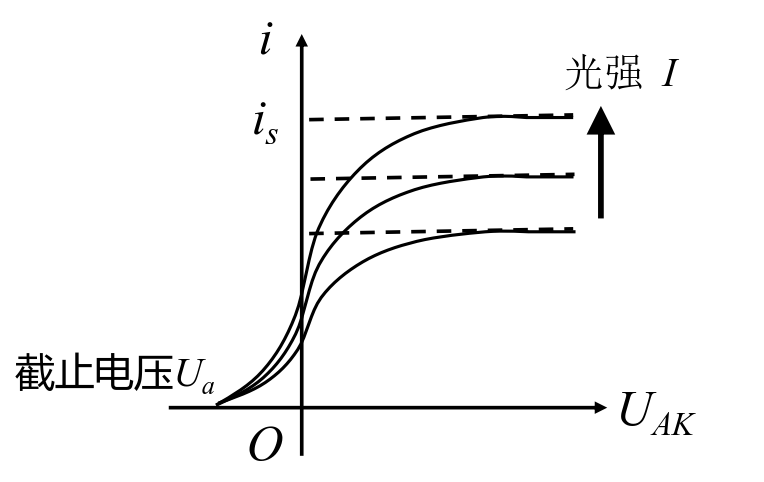
\includegraphics[width=\textwidth]{figures/图片2.png} 
            \caption{光电效应伏安特性曲线}
            \label{fig:left}
        \end{subfigure}
        %\hfill % 这是一个弹性空格，把两张图撑开
        % 第二张图片
        \begin{subfigure}[b]{0.35\textwidth}
            \centering
            % 替换为你的第二张文件名
            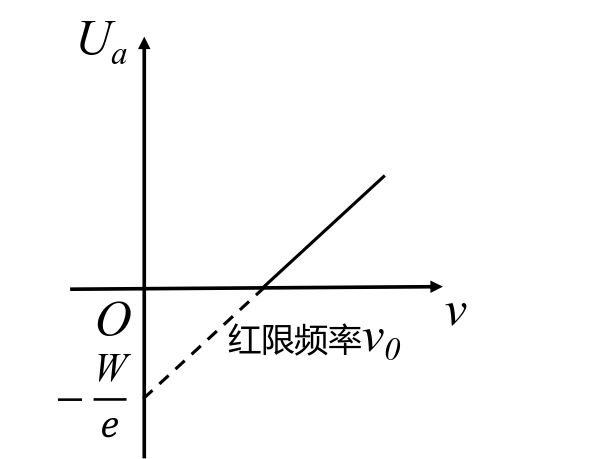
\includegraphics[width=\textwidth]{figures/图片1.png}
            \caption{光电效应截止频率与所加反向电压的关系}
            \label{fig:right}
        \end{subfigure}
        
        \label{fig:both}
    \end{figure}

    当电子逸出时，其最大初动能等于它克服电场力做的功，即\(\frac{1}{2}mv^2 = eU_a\)。
    
    由于 $U_a \propto \nu $, 与光的强度无关，所以初动能只是随着频率的增大而增大，$U_a$ 与 $\nu $ 的关系可用爱因斯坦方程表示：\(U_a = \frac{h}{e}\nu - \frac{W_0}{e}\)（其中\(W_0\)为阴极材料的逸出功）。
    
    实验时用不同频率的单色光（\(\nu_1, \nu_2, \cdots\)）照射阴极，测出相对应的遏止电位差（\(U_{a1}, U_{a2}, \cdots\)），然后画出\(U_a - \nu\)图，此图斜率\(k = \frac{h}{e}\)，由此得：\(h = ke\)。
    
    本实验成功关键在于正确地确定遏止电压差，画出\(U_a - \nu\)图，而实际测量中如何正确地确定遏止电位差，还要根据使用的光电管来决定。
    
    \subsubsection*{实验内容:}

    \textbf{测试前准备：}将 FB807 测试仪及汞灯电源接通，预热 20 分钟，调整光电管与汞灯距离约为 30-40cm，并保持不变。用专用连接线将光电管暗箱电输入端与 FB807 测试仪后面板上电压输出线连接起来，将 “电流量程” 选择开关置于合适档位。测试仪在开机或改变电流量程后，都需进行调零。调零时，应将光电信号开关按下，旋转 “调零” 旋钮使电流表为 0。调好后，将光电开关释放。
    
    \textbf{用 FB807 实验仪测定截止电压、伏安特性：}本实验仪器的电流放大器灵敏度高，稳定性好，光电管阳极反向电流、暗电流水平也较低，在测量各谱线的截止电压 $U_a$ 时，可采用零电流法（即交点法），即直接将各谱线照射下测得的电流为零时对应的电压 $U_{AK}$ 的绝对值作为截止电压 $U_a$。
    
    (1)测量截止电压：
    
    将工作电压转换至 “$-4.5—+ 2.5V $档”，“电流量程” 开关置于\(10^{-13}A\)档，光电信号开关置于关，对电流测量调零；再将$ 365nm $的滤色片转到窗口（通光口），此时把电压表显示的 $U_{AK}$ 值调整到$ - 1.999V$，打开汞灯遮光盖，电流表显示对应的电流$I$应为负值。用电压粗调和细调旋钮，逐步升高工作电压（即使负电压绝对值减小），当电压到达某一数值时，光电管输出电流为零，记录对应的工作电压 $U_{AK}$，该电压即为 $365nm$ 单色光的遏止电位。然后，按顺序依次换上 $405nm$、$436nm$、$546nm$、$577nm$ 的滤色片，重复以上测量步骤，将各 $U_{AK}$ 值记入表中。

    (2)测光电管的伏安特性曲线:

    此时，将工作电压转换置:$-4.5—+30V$，“电流量程”开关转换至\(10^{-10}A\)档，并重新调零。其余操作步骤与“测量截止电压”同，不过此时要把每一个工作电压和对应的电流值加以记录，以便画出饱和伏安特性曲线，并对该特性进行研究分析。

    观察在同一光阑、同一距离条件下 5 条伏安特性曲线。记录所测  $U_{AK}$ 及 $I$的数据到表中，在座标纸上作对应于以上波长及光强的伏安特性曲线。
    
    观察同一距离、不同光阑（不同光通量）、某条谱线在的饱和伏安特性曲线。测量并记录对同一谱线、同一入射距离，而光阑分别为 $2mm,4mm,8mm$时对应的电流值于表中，验证光电管的饱和光电流与入射光强成正比。

    观察同一光阑下、不同距离（不同光强）、某条谱线在的饱和伏安特性曲线。在 $U_{AK}$ 为 30V 时，测量并记录对同一谱线、同一光阑时，光电管与入射光在不同距
离，如 $300mm,350mm,400mm$等对应的电流值于表中，同样可以验证光电管的饱
和电流与入射光强成正比。


    
    \textbf{普朗克常数 $h$ 的计算：}由表中数据，画出\(U_a - \nu\)图，求出直线的斜率 $k$，即可用\(h = ek\)求出普朗克常数 $h$，将其与公认值\(h_0\)比较，求出相对误差：\(E = \frac{|h - h_0|}{h_0}×100\%\)。
    
    \subsection{实验重点}

    \xiaosi（简述本实验的学习重点，不超过100字，3分）


    \begin{enumerate}   
        \item 了解光电效应的基本规律，验证爱因斯坦光电效应方程；
        \item 掌握用光电效应法测定普朗克常数 $h$。
    \end{enumerate}  
    
    
    \subsection{实验难点}
    
    \xiaosi（简述本实验的实现难点，不超过100字，2分）

    \begin{enumerate}    
        \item 精准测定遏止电压，需排除暗电流、阳极反向电流干扰；
        \item 仪器读数易受温度漂移影响，稳定性难把控；
        \item 滤光片实际透光波长与标称值有偏差，汞灯光强不稳定；
        \item 绘制 $U_a-\nu$ 图并拟合直线求斜率，需保证数据准确性以减小误差。
    \end{enumerate} 

    \

\section{原始数据}

    \xiaosi （将有老师签名的“自备数据记录草稿纸”的扫描或手机拍摄图粘贴在下方，20分）

    \begin{figure}[htbp]
        \centering
        % 第一张图片
        \begin{subfigure}[b]{0.48\textwidth}
            \centering
            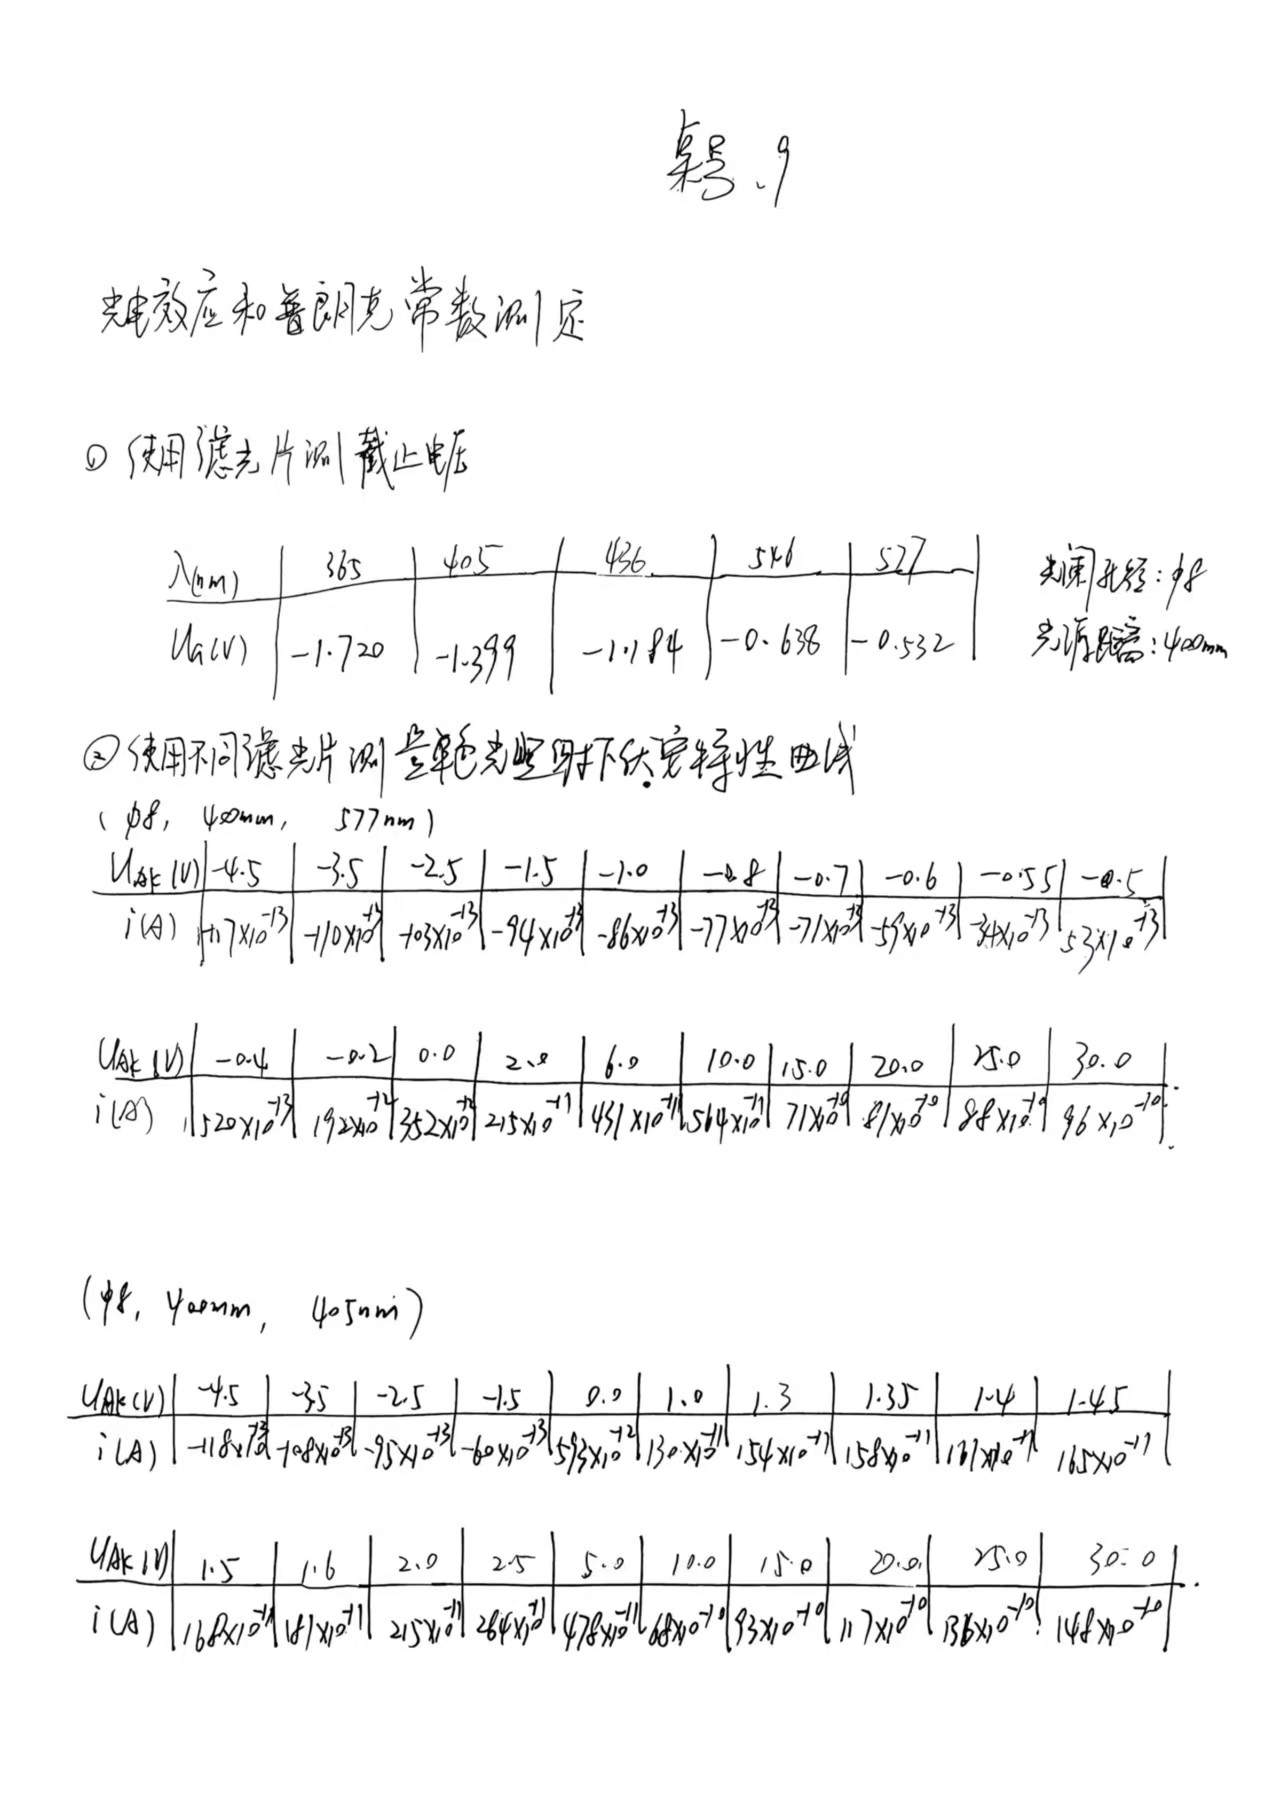
\includegraphics[width=\textwidth]{figures/实验数据-1.jpg} 
            \label{fig:left}
        \end{subfigure}
        %\hfill % 这是一个弹性空格，把两张图撑开
        % 第二张图片
        \begin{subfigure}[b]{0.48\textwidth}
            \centering
            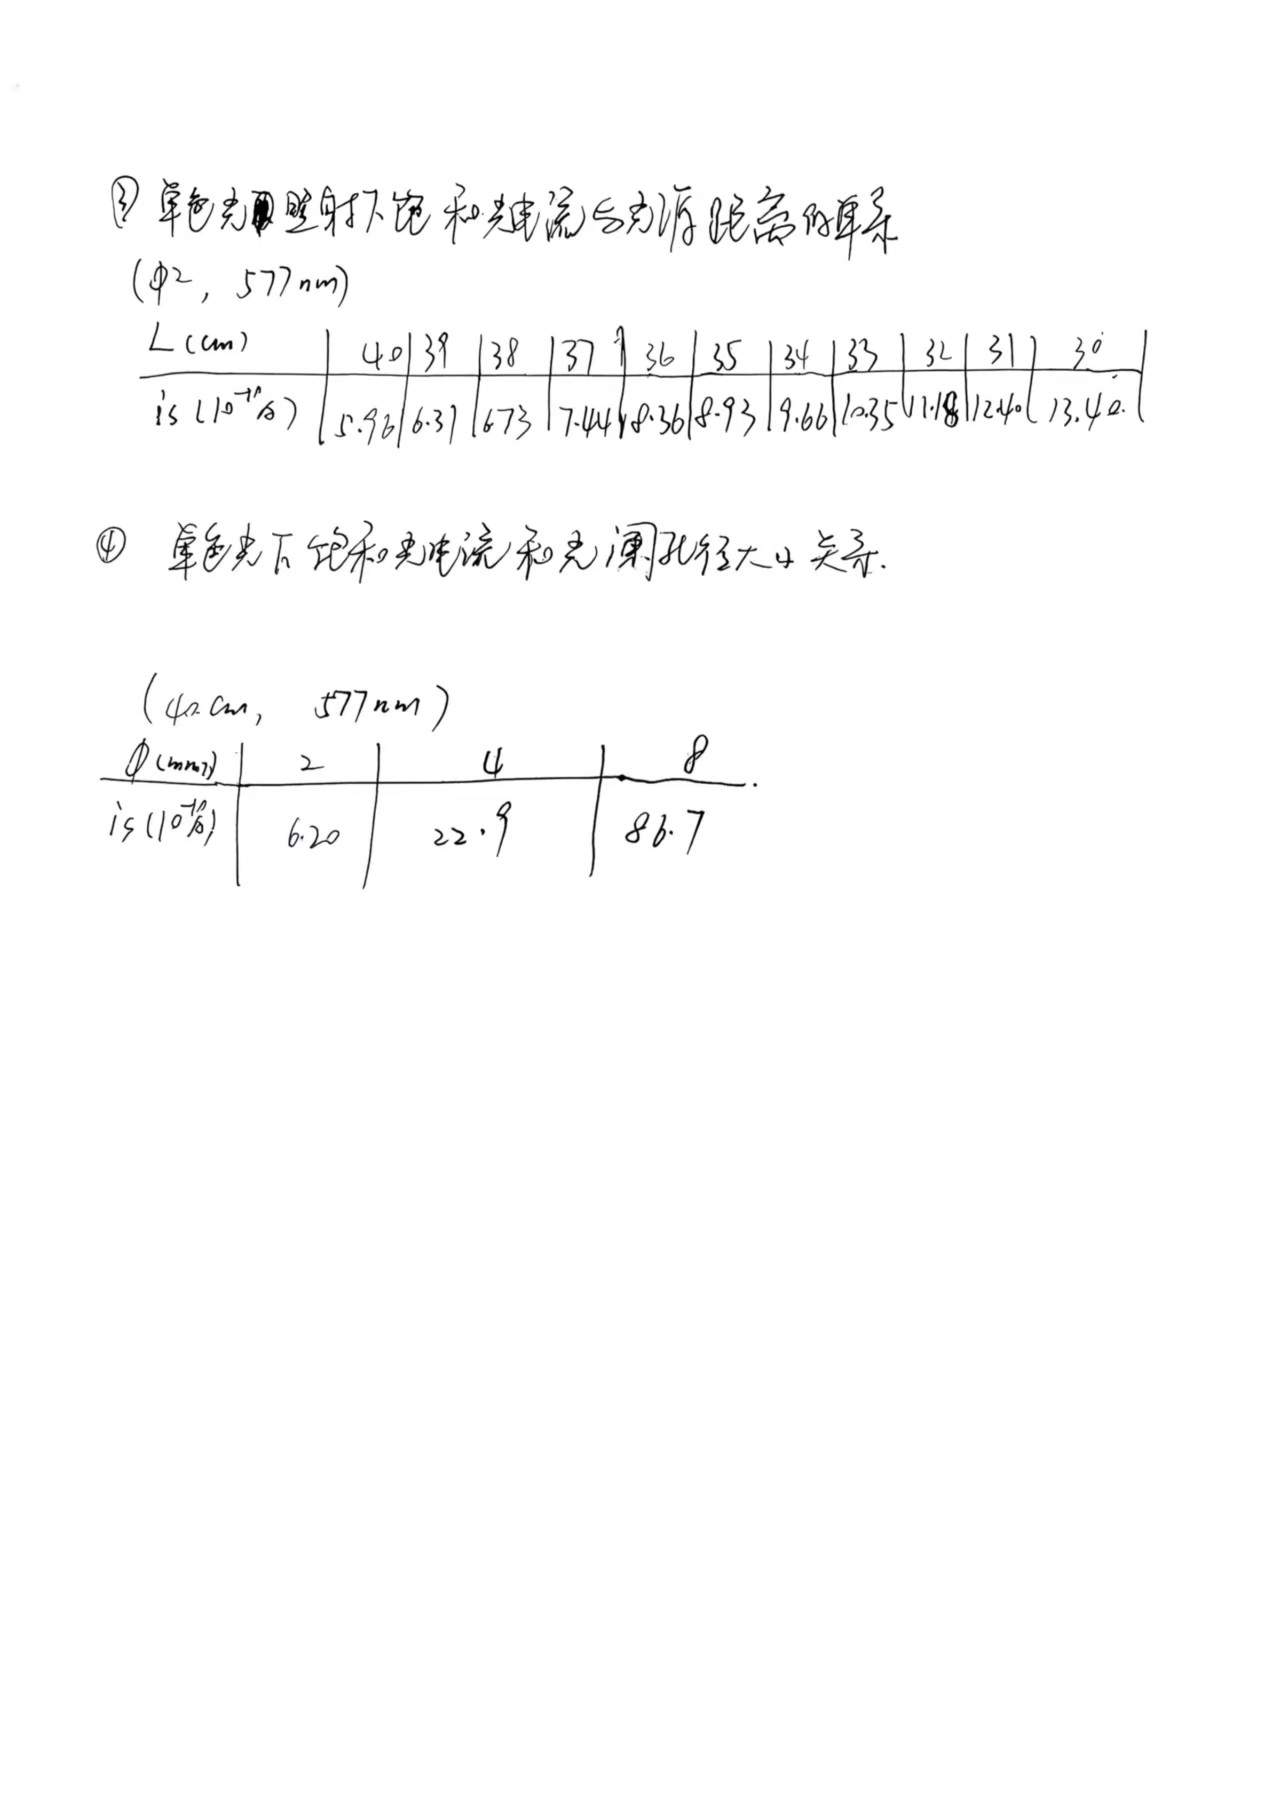
\includegraphics[width=\textwidth]{figures/实验数据-2.jpg}
            \label{fig:right}
        \end{subfigure}
        
        \caption{实验数据}
        \label{fig:both}
    \end{figure}

\newpage
    
\section{结果与分析}

    \subsection{数据处理与结果}
    \xiaosi （列出数据表格、选择数据处理方法、给定测量或计算结果，30分）
    
    \

    
    \subsubsection{测量截止电压：}

    \begin{table}[H]
    \centering
    \caption{使用滤光片测截止电压 ($\phi 8$, 光源距离 400mm)}
    \begin{tabular}{cccccc}
        \toprule
        $\lambda$ (nm) & 365 & 405 & 436 & 546 & 577 \\
        \midrule
        $U_a$ (V) & -1.720 & -1.399 & -1.184 & -0.638 & -0.532 \\
        \bottomrule
    \end{tabular}
\end{table}

对上表中数据进行线性拟合，得到如下图直线：

\begin{figure}[H]
        \centering
        % 第一张图片
            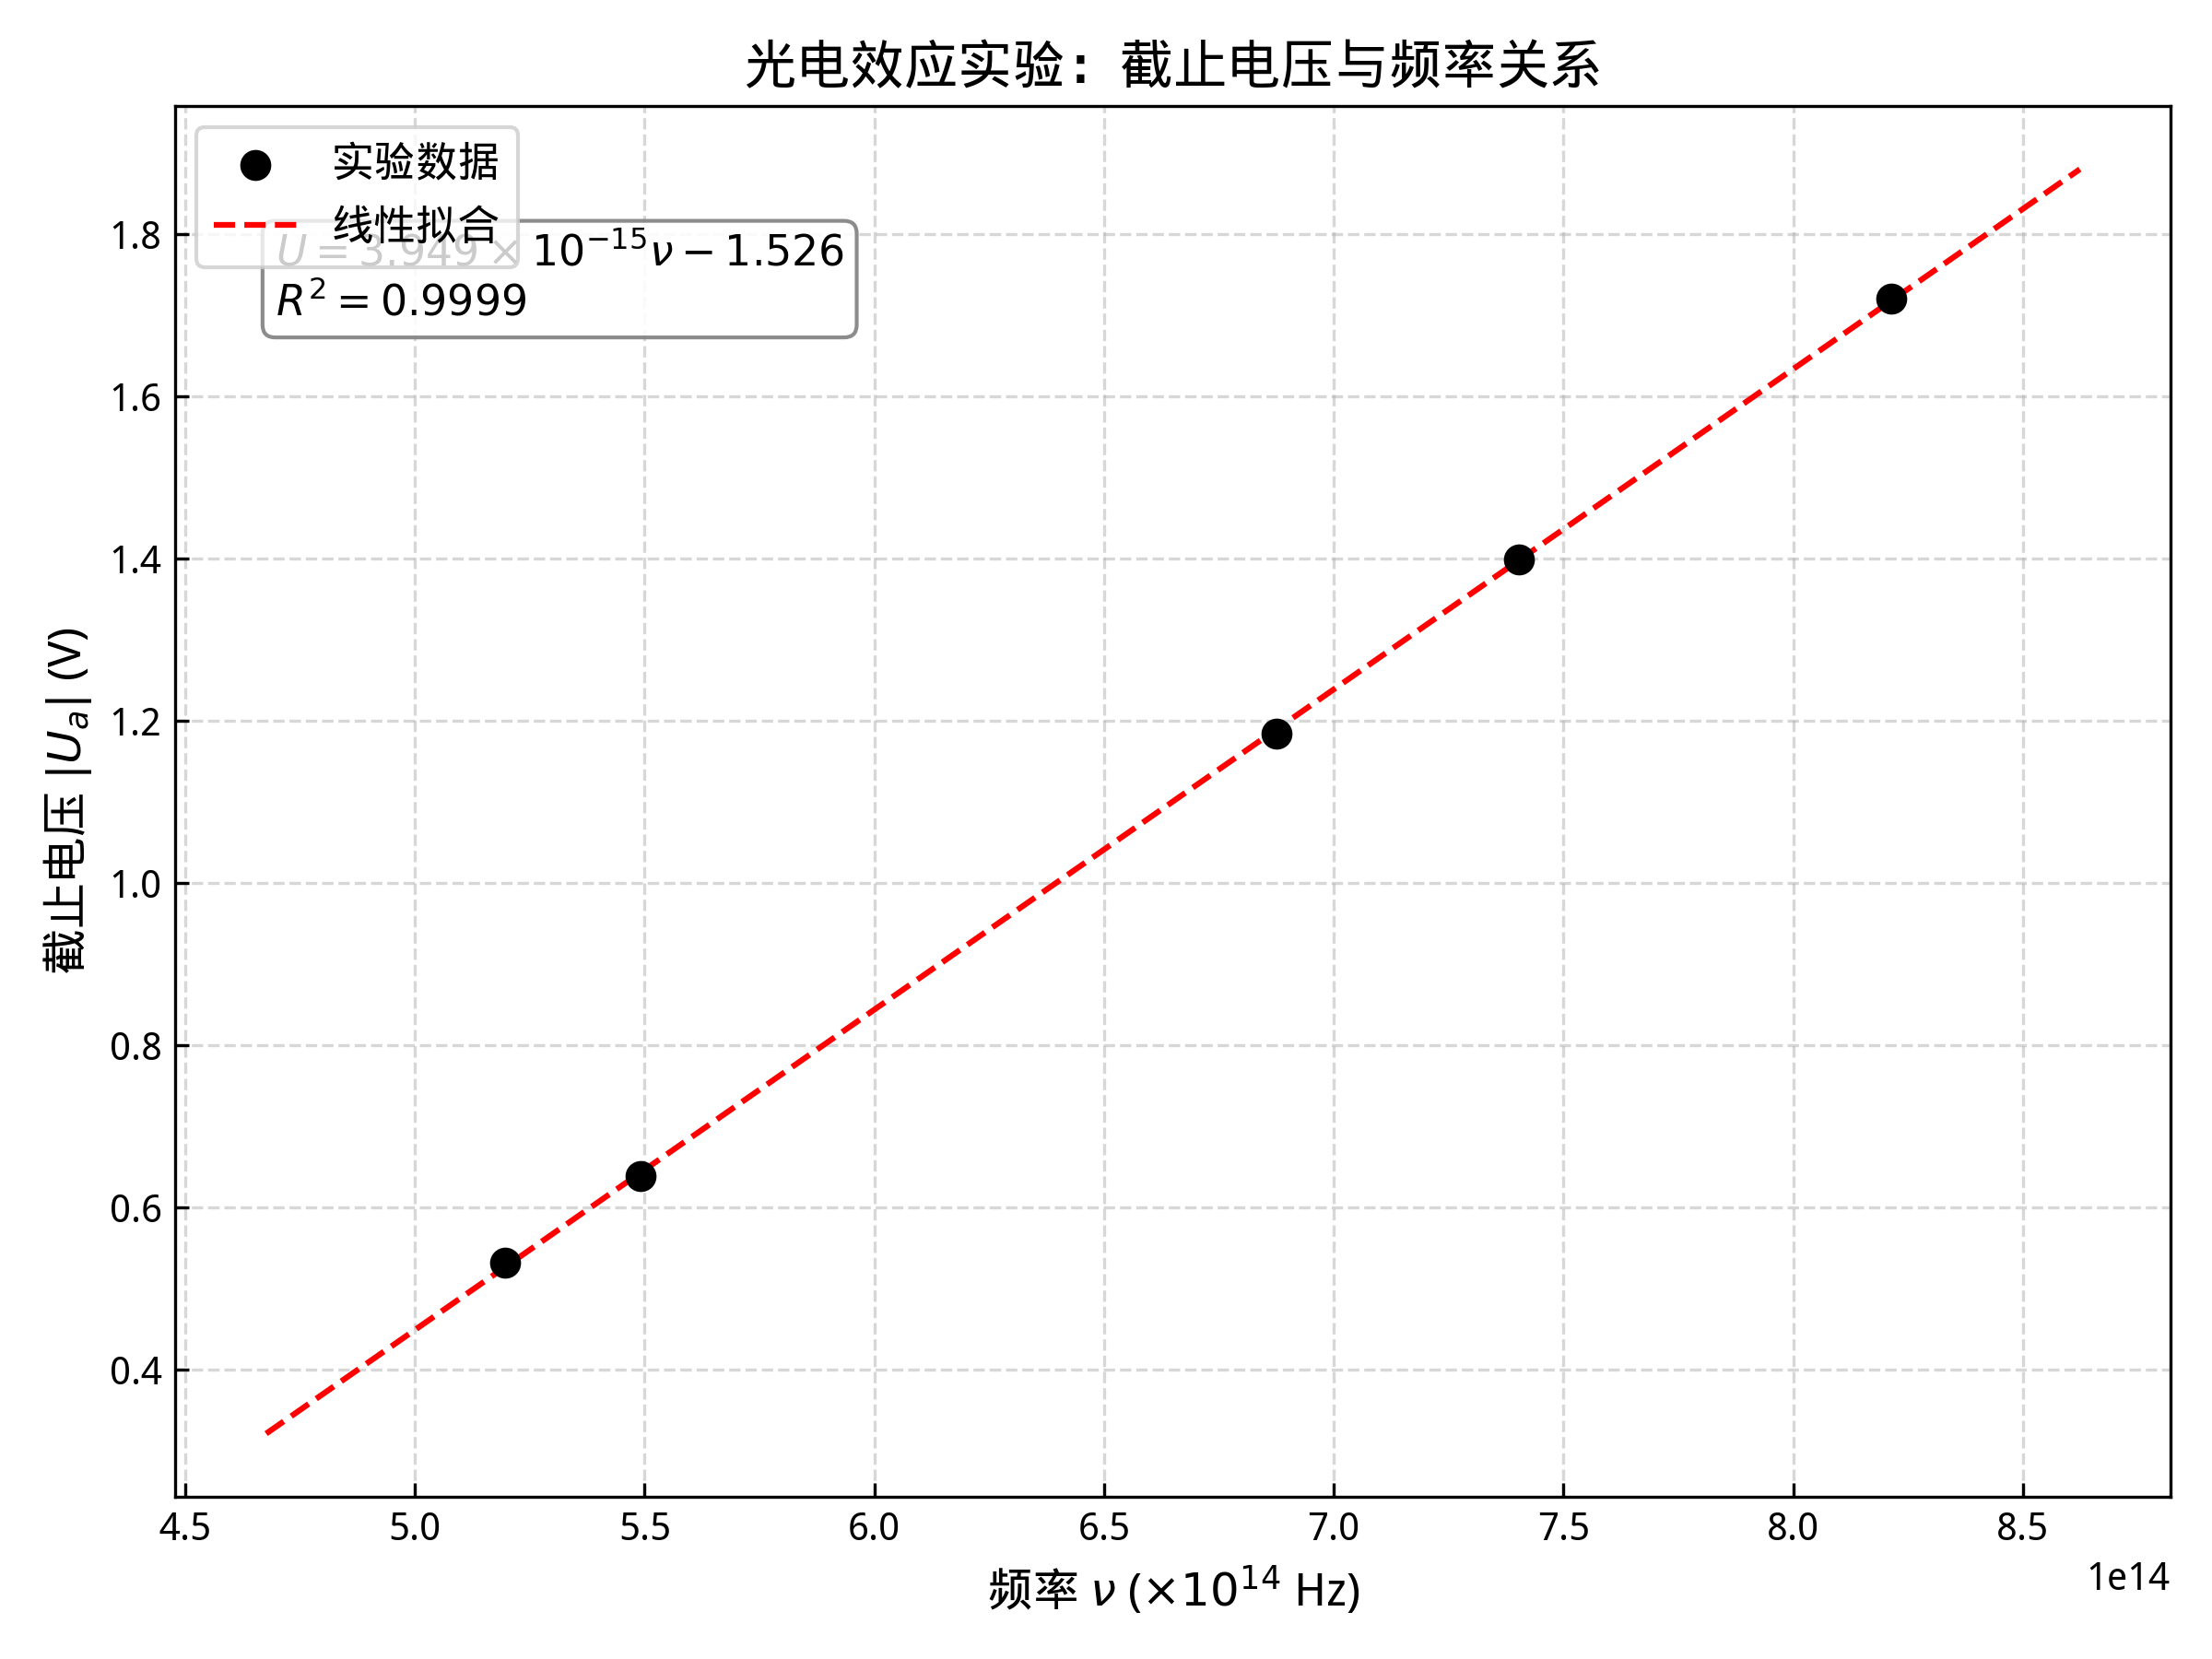
\includegraphics[width=14cm]{figures/photoelectric_fit.png} 
            \label{fig:left}
    \end{figure}

    根据光电效应方程 $eU_a = h\nu - W$，整理得截止电压 $U_a$ 与频率 $\nu$ 的线性关系：
\begin{equation*}
    U_a = \frac{h}{e}\nu - \frac{W}{e} = k\nu + b
\end{equation*}
其中，斜率 $k = \frac{h}{e}$，截距 $b = -\frac{W}{e}$。

将实验测得的波长 $\lambda$ 转换为频率 $\nu = \frac{c}{\lambda}$，并对 $( \nu, |U_a| )$ 数据点进行最小二乘法线性拟合。实验数据处理及拟合结果如下：

\begin{itemize}
    \item 拟合方程：$U_a = 4.044 \times 10^{-15} \nu - 1.589$
    \item 线性相关系数：$R^2 = 0.9992$
    \item 斜率 $k = (4.044 \pm 0.063) \times 10^{-15} \, \text{V}\cdot\text{s}$
    \item 截距 $b = -1.589 \pm 0.421 \, \text{V}$
\end{itemize}


已知元电荷 $e = 1.602 \times 10^{-19} \, \text{C}$，光速 $c = 2.998 \times 10^{8} \, \text{m/s}$。

\vspace{0.3cm}
\noindent\textbf{1. 普朗克常数$h$的计算与不确定度分析 }

根据斜率 $k$ 计算普朗克常数及其不确定度：
\begin{align*}
    h_{\text{meas}} &= k \cdot e = 4.044 \times 10^{-15} \times 1.602 \times 10^{-19} = 6.479 \times 10^{-34} \, \text{J}\cdot\text{s} \\
    u_h &= u_k \cdot e = 0.063 \times 10^{-15} \times 1.602 \times 10^{-19} = 1.01 \times 10^{-35} \, \text{J}\cdot\text{s}
\end{align*}
结果表示为：
\begin{equation*}
    h = (6.48 \pm 0.10) \times 10^{-34} \, \text{J}\cdot\text{s}
\end{equation*}

\vspace{0.3cm}
\noindent\textbf{2. 逸出功 $W$的计算与不确定度分析}

根据截距 $b$ 计算材料的逸出功：
\begin{align*}
    W &= -b \cdot e = -(-1.589) \, \text{eV} = 1.59 \, \text{eV} \\
    W_{\text{J}} &= 1.59 \times 1.602 \times 10^{-19} = 2.55 \times 10^{-19} \, \text{J}
\end{align*}
其不确定度为 $u_W = u_b \cdot e \approx 0.067 \times 10^{-19} \, \text{J}$。

\vspace{0.3cm}
\noindent\textbf{3. 红限频率 $\nu_0$的计算与不确定度分析}

当 $U_a = 0$ 时对应的频率即为红限频率：
\begin{equation*}
    \nu_0 = -\frac{b}{k} = \frac{1.589}{4.044 \times 10^{-15}} = 3.929 \times 10^{14} \, \text{Hz}
\end{equation*}
根据误差传递公式 $u_{\nu_0} = \nu_0 \sqrt{(u_b/b)^2 + (u_k/k)^2}$ 计算得 $u_{\nu_0} \approx 0.12 \times 10^{14} \, \text{Hz}$。

\noindent\textbf{4. 相对误差分析}

普朗克常数的公认值 $h_{\text{ref}} = 6.626 \times 10^{-34} \, \text{J}\cdot\text{s}$。本实验的相对不确定度（相对误差）为：
\begin{equation*}
    E_r = \frac{|h_{\text{meas}} - h_{\text{ref}}|}{h_{\text{ref}}} \times 100\% = \frac{|6.479 - 6.626|}{6.626} \times 100\% = 2.22\%
\end{equation*}

\subsubsection{测光电管的伏安特性曲线：}

\begin{table}[H]
    \centering
    \caption{577nm 单色光下伏安特性曲线 ($\phi 8$, 400mm)}
    % 第一部分数据：负向电压区域
    \begin{tabular}{ccccccc}
        \toprule
        $U_{AK}$ (V) & -4.5 & -3.5 & -2.5 & -1.5 & -1.0 & -0.8   \\
        \midrule
        $i$ (A) & $-117\times10^{-13}$ & $-110\times10^{-13}$ & $-103\times10^{-13}$ & $-94\times10^{-13}$ & $-86\times10^{-13}$ & $-77\times10^{-13}$   \\
        \bottomrule
        $U_{AK}$ (V) & -0.7 & -0.6 & -0.55 & -0.5 & -0.4 & -0.2 \\
        \midrule
        $i$ (V)  & $-71\times10^{-13}$  & $-59\times10^{-13}$ & $-34\times10^{-13}$ & $53\times10^{-13}$ & $520\times10^{-13}$ & $192\times10^{-12}$\\
        \bottomrule
        $U_{AK}$ (V) & 0.0 & 2.0 & 6.0 & 10.0  & 15.0 & 20.0 \\
        \midrule
        $i$ (A)  & $352\times10^{-12}$ & $215\times10^{-11}$ & $431\times10^{-11}$ & $564\times10^{-11}$ & $71\times10^{-10}$ & $81\times10^{-10}$ \\
        \bottomrule
        $U_{AK}$ (V)  & 25.0 & 30.0 \\
        \midrule
        $i$ (A)  & $88\times10^{-10}$ & $96\times10^{-10}$ \\
        \bottomrule
    \end{tabular}
\end{table}

对上表中数据进行拟合，得到如下图曲线：

\begin{figure}[H]
        \centering
        % 第一张图片
            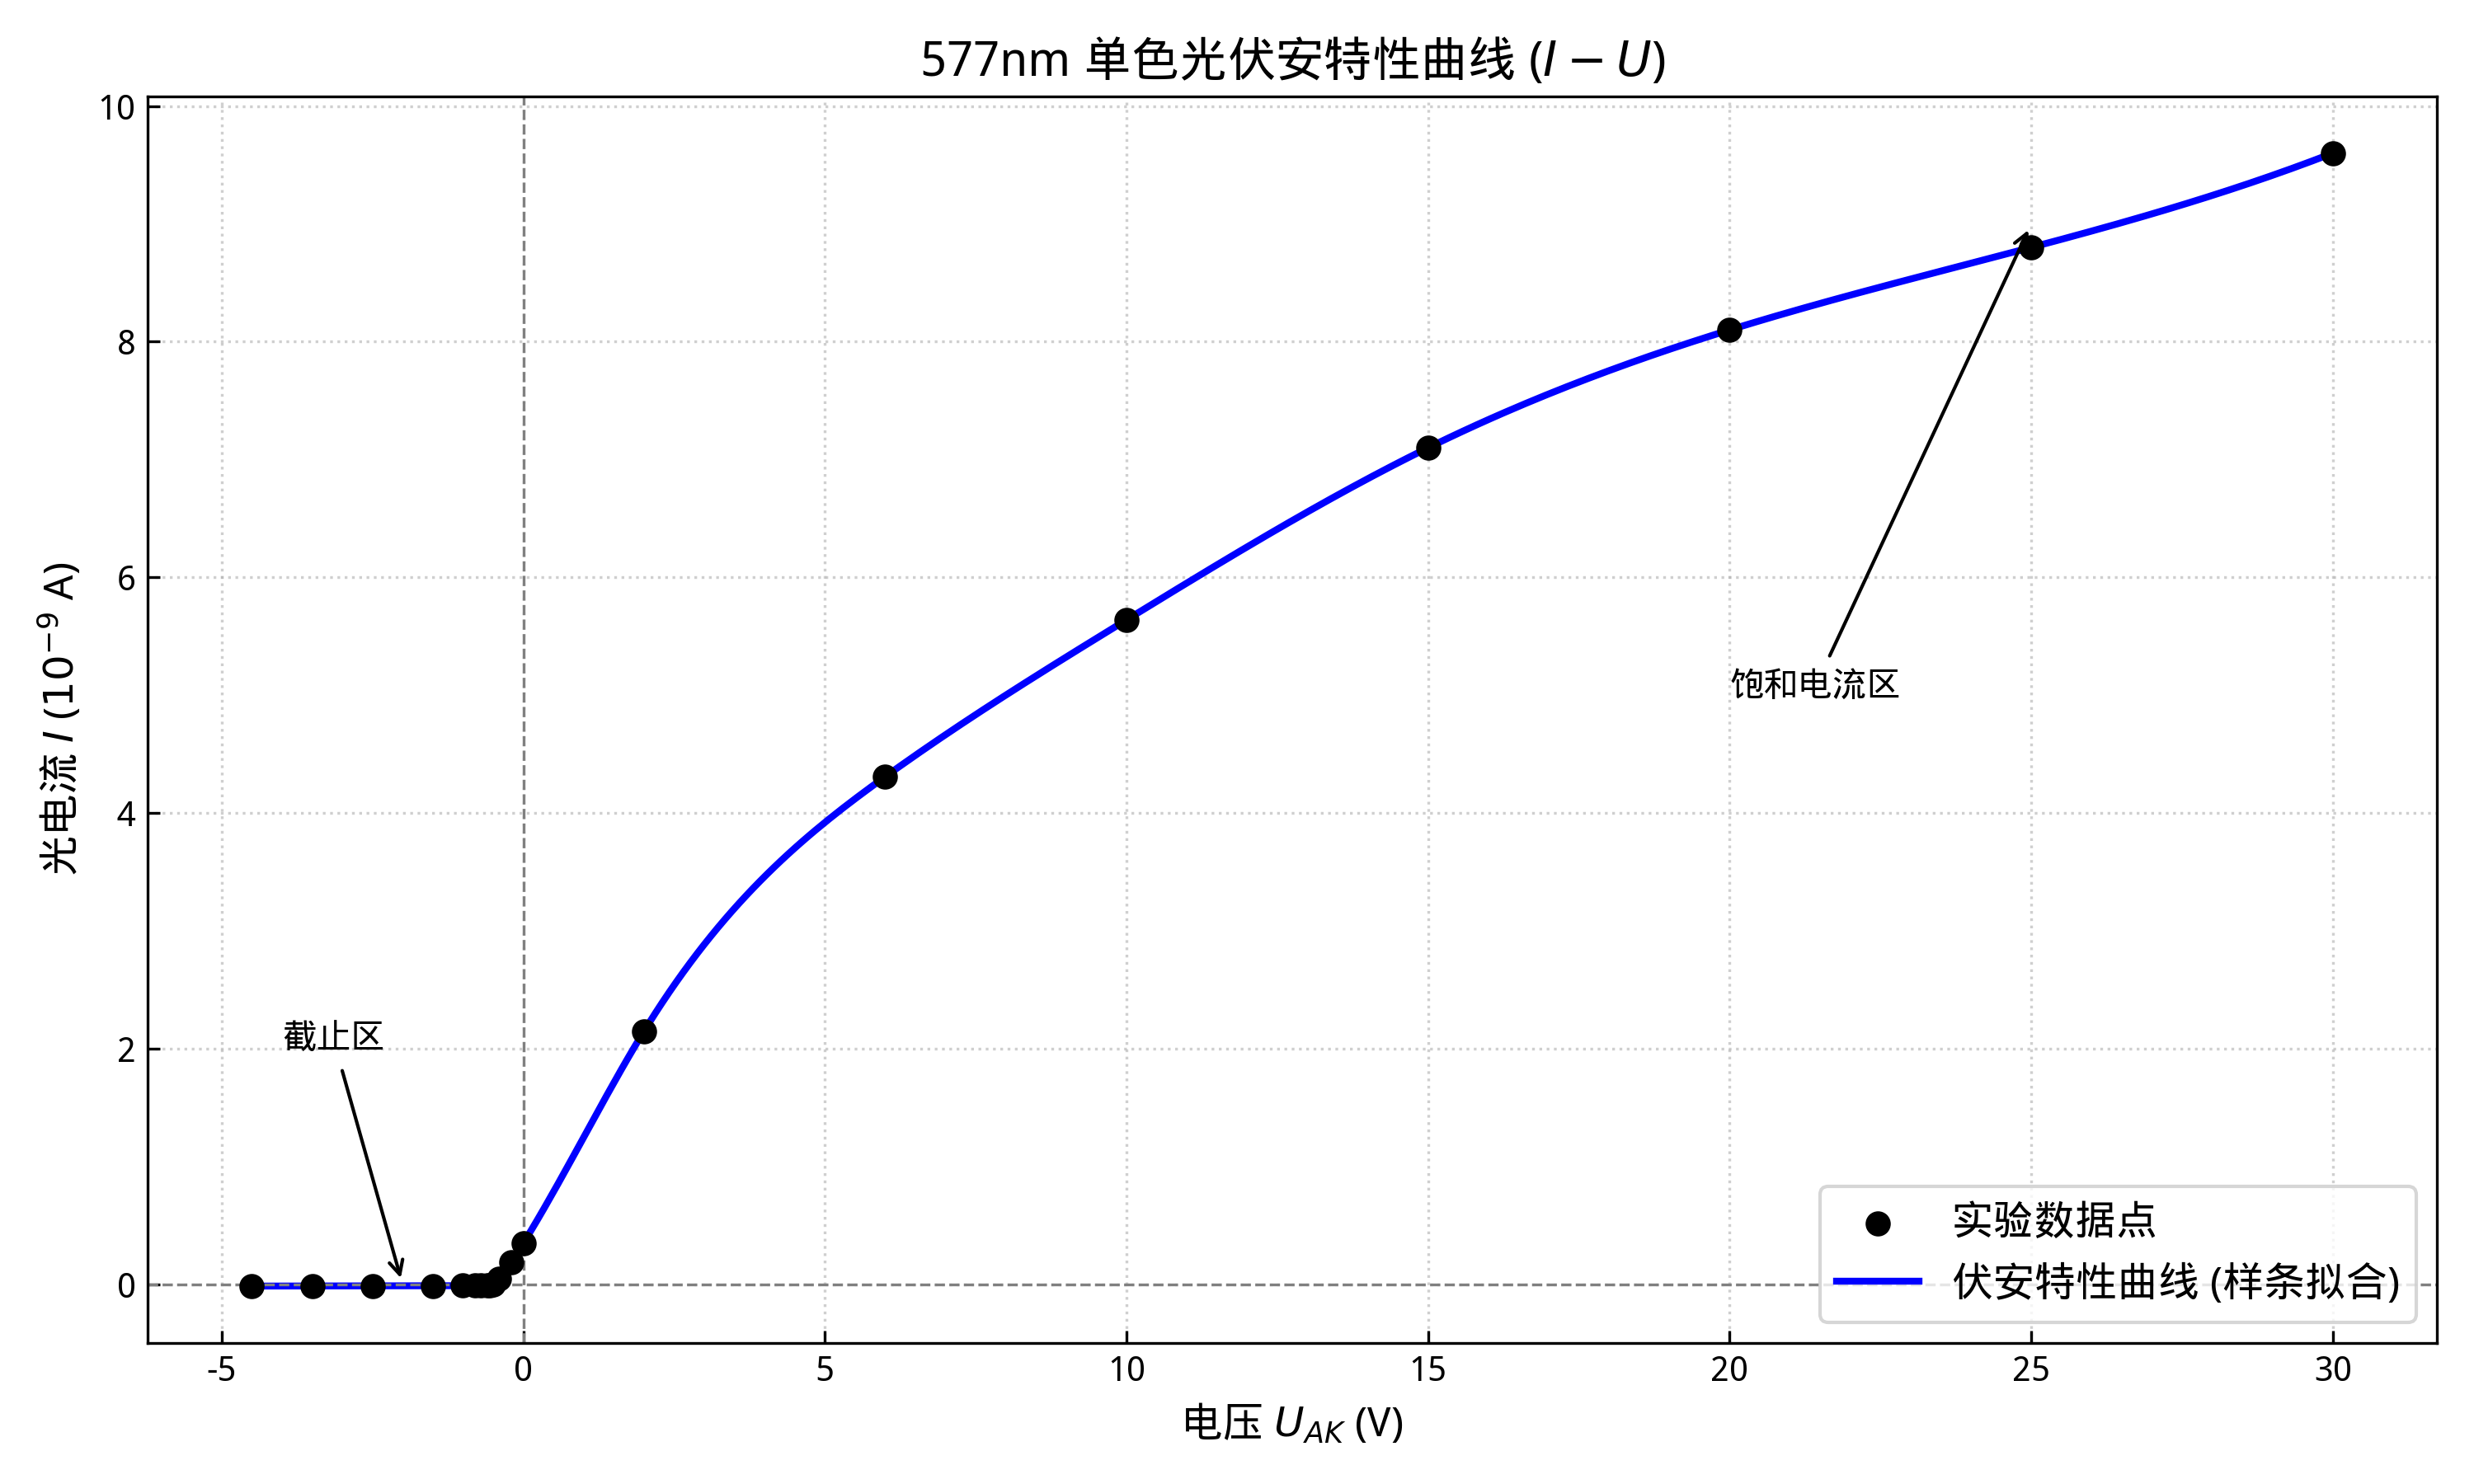
\includegraphics[width=14cm]{figures/iv_curve_smooth.png} 
            \label{fig:left}
    \end{figure}

\begin{table}[H]
    \centering
    \caption{405nm 单色光下伏安特性曲线 ($\phi 8$, 400mm)}
    \begin{tabular}{ccccccc}
        \toprule
        % 第一组：负压及过零点
        $U_{AK}$ (V) & -4.5 & -3.5 & -2.5 & -1.5 & 0.0 & 1.0 \\
        \midrule
        $i$ (A) & $-118\times10^{-13}$ & $-108\times10^{-13}$ & $-95\times10^{-13}$ & $-60\times10^{-13}$ & $593\times10^{-12}$ & $130\times10^{-11}$ \\
        \bottomrule
        
        % 第二组：正压细分区域
        $U_{AK}$ (V) & 1.3 & 1.35 & 1.4 & 1.45 & 1.5 & 1.6 \\
        \midrule
        $i$ (A) & $154\times10^{-11}$ & $158\times10^{-11}$ & $161\times10^{-11}$ & $165\times10^{-11}$ & $168\times10^{-11}$ & $181\times10^{-11}$ \\
        \bottomrule
        
        % 第三组：正压上升区域
        $U_{AK}$ (V) & 2.0 & 2.5 & 5.0 & 10.0 & 15.0 & 20.0 \\
        \midrule
        $i$ (A) & $215\times10^{-11}$ & $264\times10^{-11}$ & $478\times10^{-11}$ & $68\times10^{-10}$ & $93\times10^{-10}$ & $117\times10^{-10}$ \\
        \bottomrule
        
        % 第四组：尾部数据
        $U_{AK}$ (V) & 25.0 & 30.0 \\
        \midrule
        $i$ (A) & $136\times10^{-10}$ & $148\times10^{-10}$ \\
        \bottomrule
    \end{tabular}
\end{table}

对上表中数据进行拟合，得到如下图曲线：

\begin{figure}[H]
        \centering
        % 第一张图片
            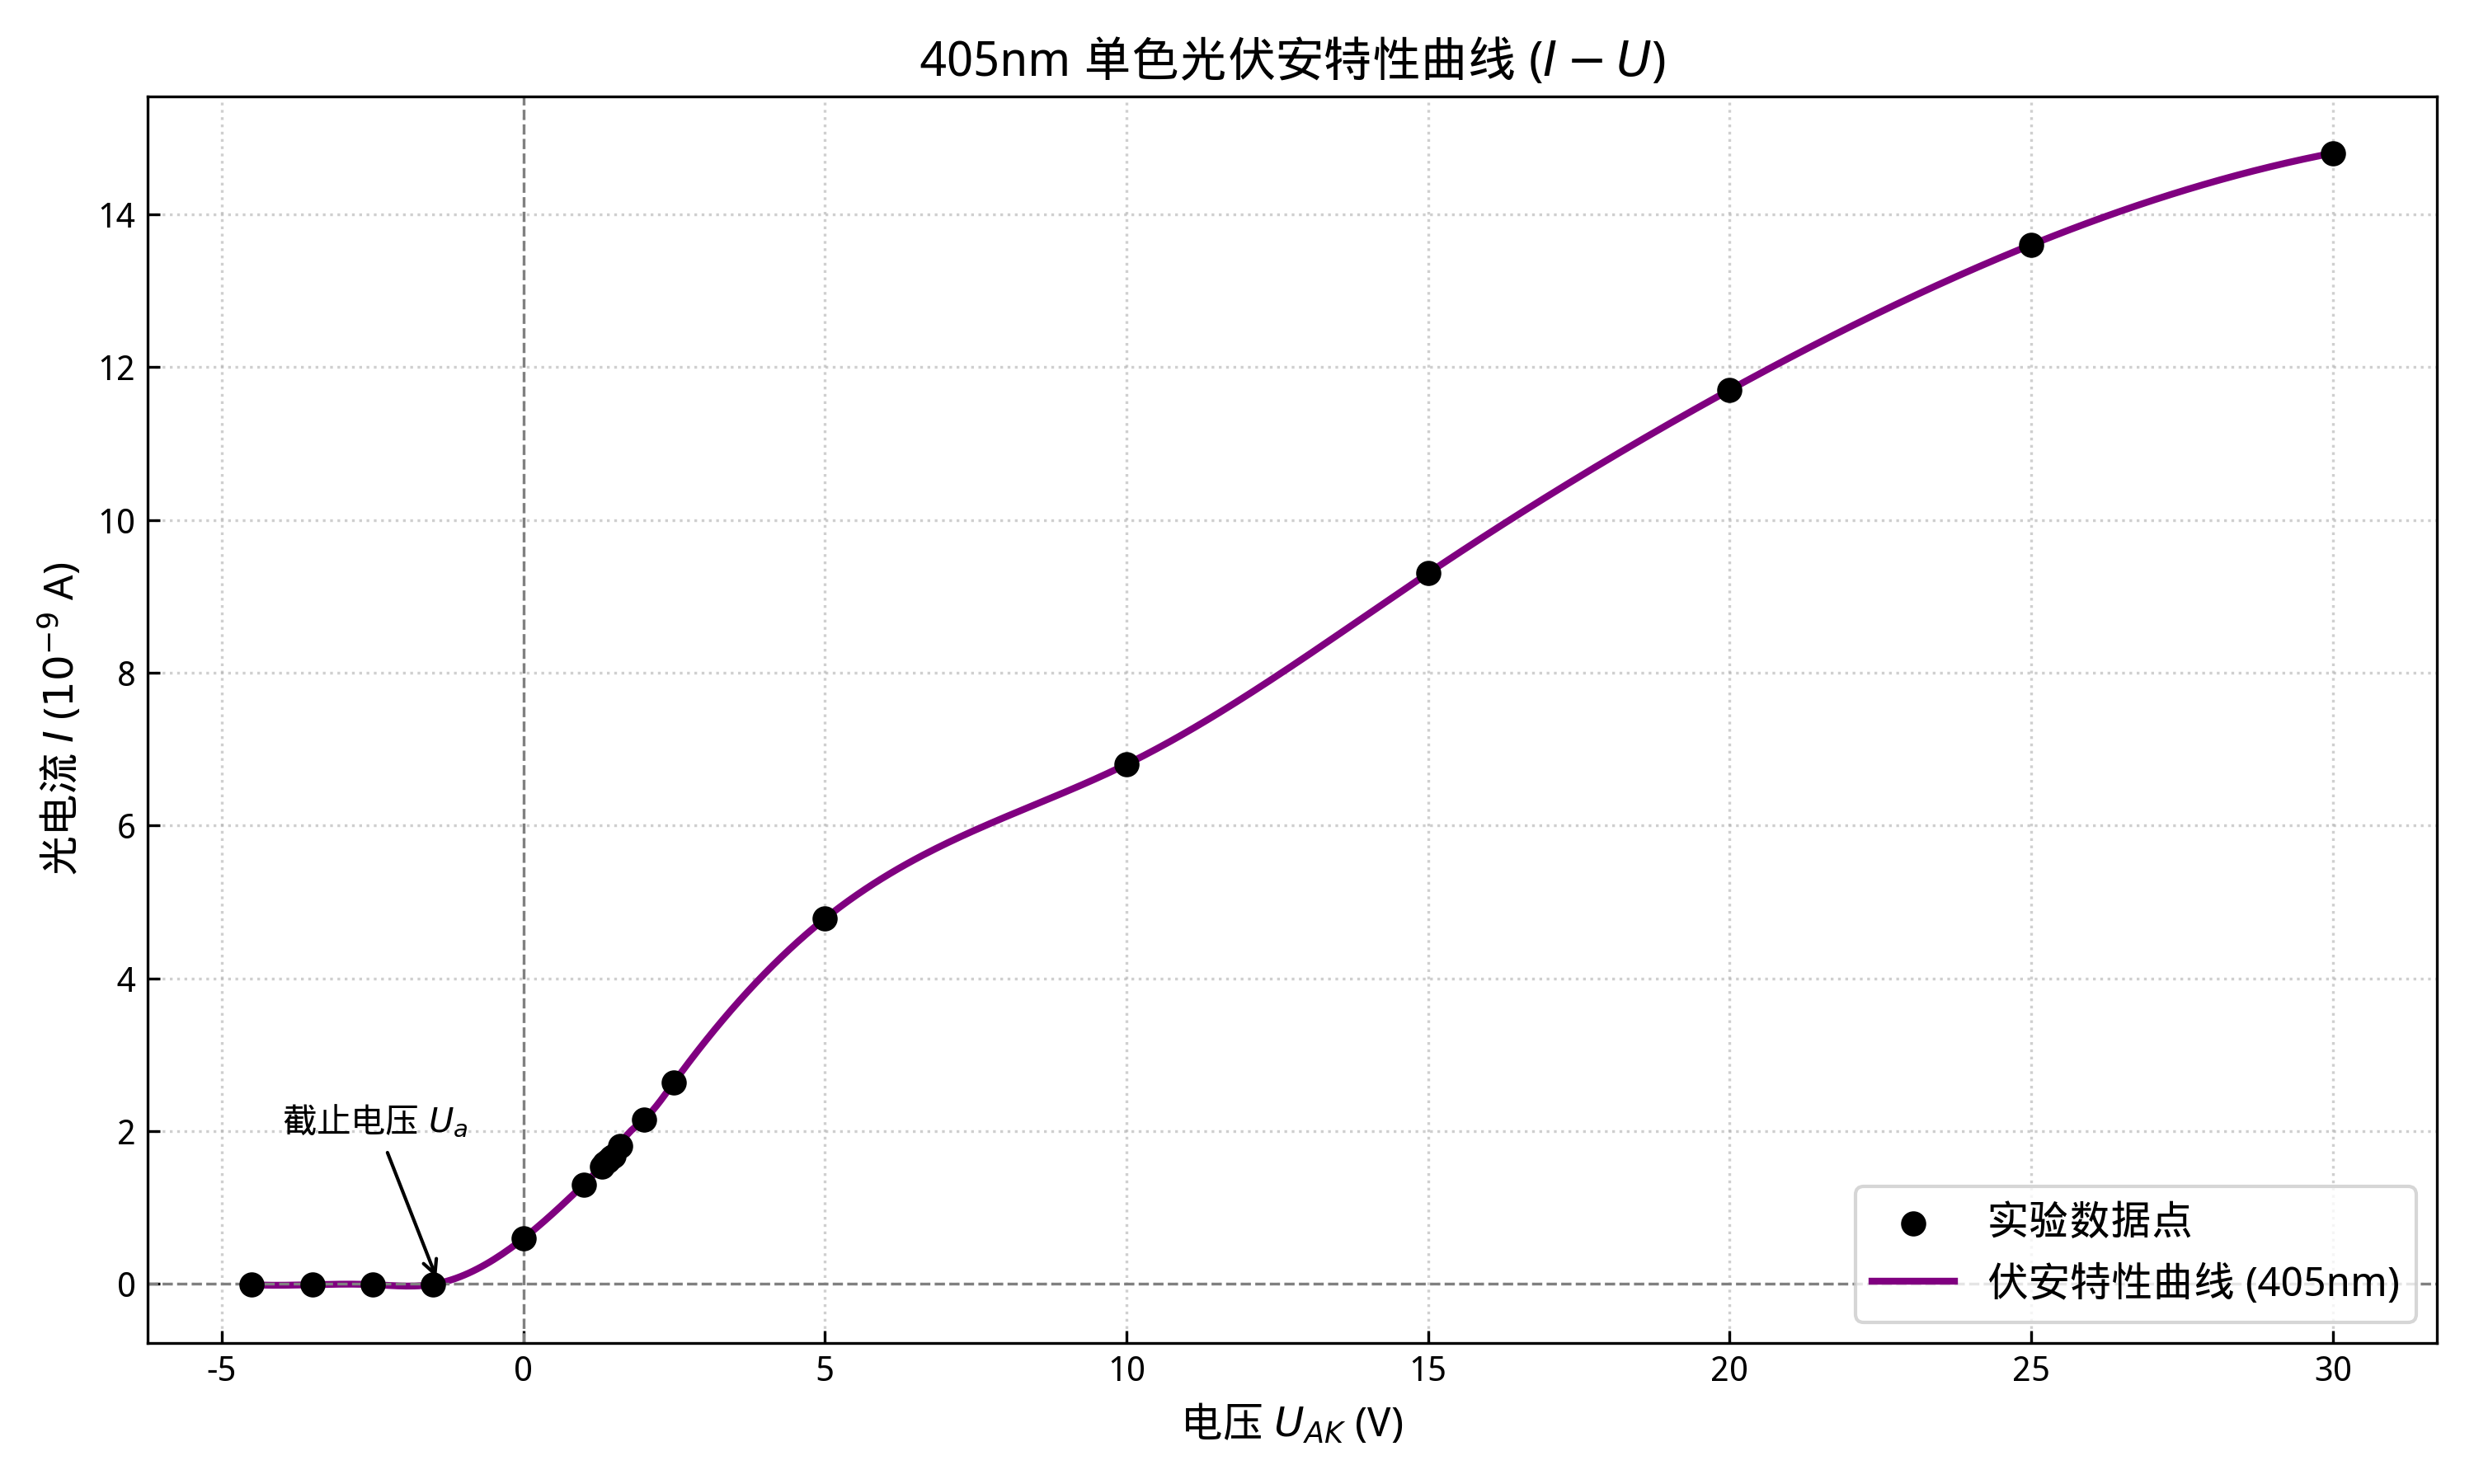
\includegraphics[width=14cm]{figures/iv_curve_405_smooth.png} 
            \label{fig:left}
    \end{figure}

\begin{table}[H]
    \centering
    \caption{单色光照射下饱和电流与光源距离的关系 ($\phi 2, 577\text{nm}$)}
    \begin{tabular}{cccccccccccc}
        \toprule
        % 第一行数据
        $L$ (cm) & 40 & 39 & 38 & 37 & 36 & 35 & 34 & 33 & 32 & 31 & 30\\
        \midrule
        $i_S$ ($10^{-10}$A) & 5.96 & 6.31 & 6.73 & 7.44 & 8.36 & 8.93 & 9.66 & 10.35 & 11.18 & 12.40 & 13.40\\
        \bottomrule
    \end{tabular}
\end{table}


\begin{table}[H]
    \centering
    \caption{单色光下饱和电流和光阑孔径大小关系 ($40\text{cm}, 577\text{nm}$)}
    \begin{tabular}{cccc}
        \toprule
        $\Phi$ (mm) & 2 & 4 & 8 \\
        \midrule
        $i_S$ ($10^{-10}$A) & 6.20 & 22.9 & 86.7 \\
        \bottomrule
    \end{tabular}
\end{table}

\subsubsection{饱和电流与光强关系的验证}

为了验证光电管饱和电流 $i_S$ 与入射光强 $I$ 成正比这一规律，本实验分别通过改变光源距离 $L$ 和改变光阑孔径 $\Phi$ 两种方式改变光强，并使用作图法进行验证。

\textbf{1. 改变光源距离 $L$}

对于点光源，光强与距离的平方成反比，即 $I \propto 1/L^2$。若饱和电流与光强成正比，则应满足线性关系：
\begin{equation*}
    i_S = k_1 \cdot \frac{1}{L^2}
\end{equation*}
以 $1/L^2$ 为横坐标，$i_S$ 为纵坐标作图，结果如图 \ref{fig:sat_dist} 所示。

\begin{figure}[H]
    \centering
    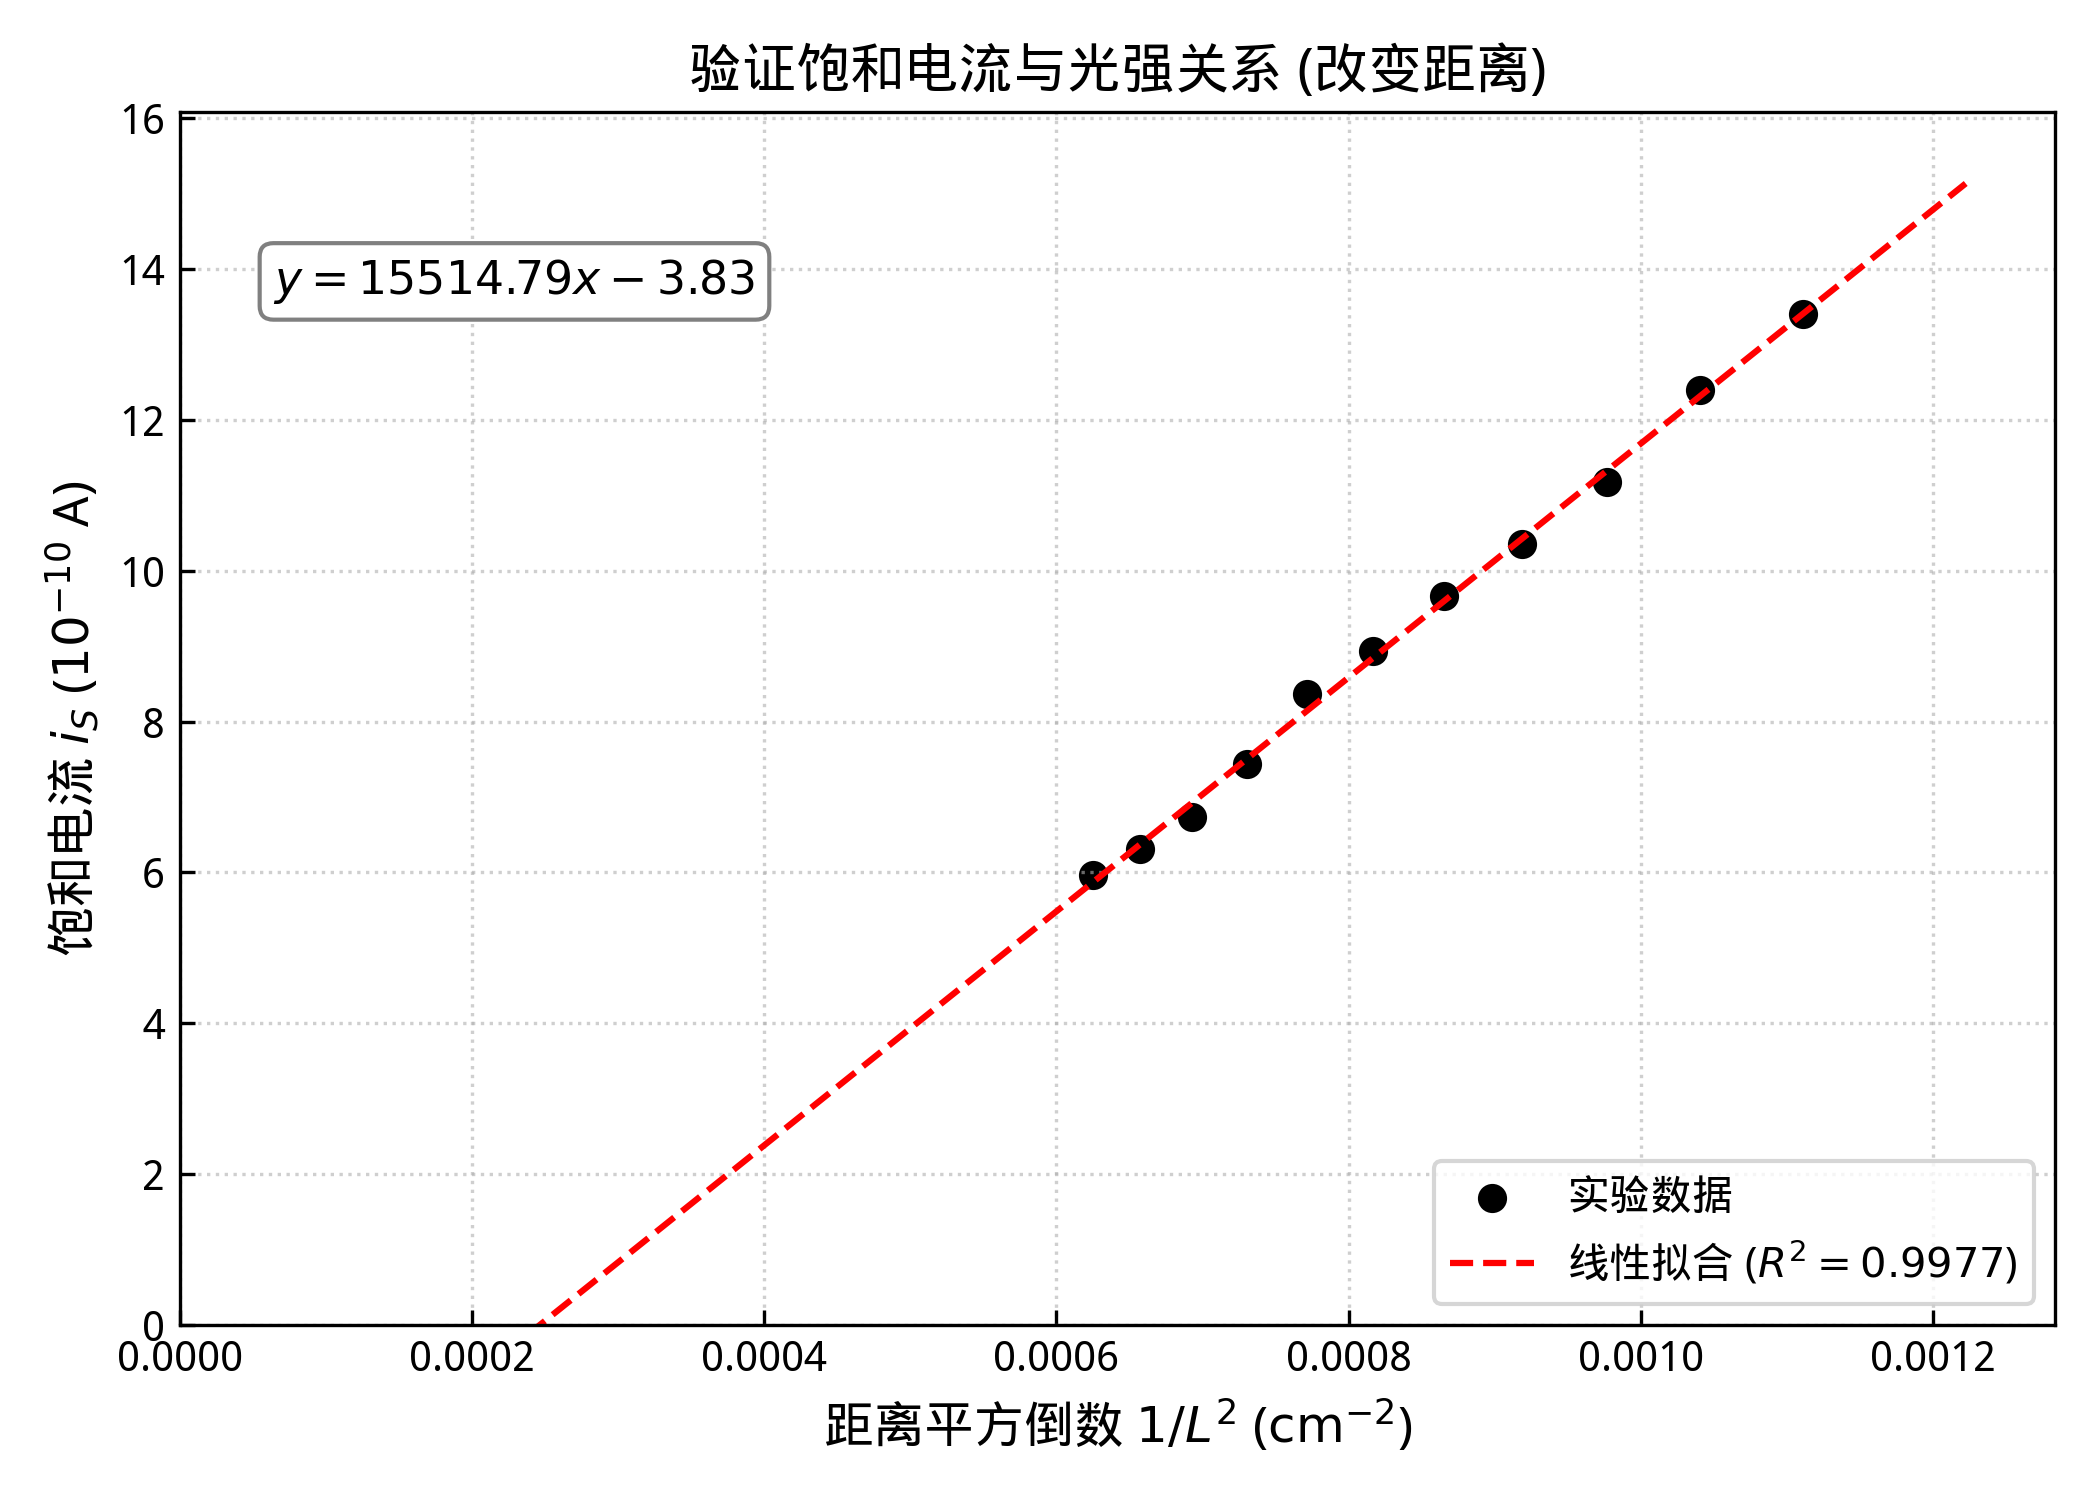
\includegraphics[width=0.8\linewidth]{./figures/saturation_distance.png}
    \caption{饱和电流 $i_S$ 与距离平方倒数 $1/L^2$ 的关系}
    \label{fig:sat_dist}
\end{figure}

由图 \ref{fig:sat_dist} 可知，数据点呈现良好的线性分布（$R^2 > 0.98$），且拟合直线近似经过原点。这表明在实验误差允许范围内，饱和电流与距离的平方成反比，即验证了 $i_S \propto I$。

\textbf{2. 改变光阑孔径 $\Phi$}

光阑控制通光面积 $S$，且 $S \propto \Phi^2$。在光源距离固定的情况下，入射光通量与孔径平方成正比。若饱和电流与光强成正比，则应满足：
\begin{equation*}
    i_S = k_2 \cdot \Phi^2
\end{equation*}
以 $\Phi^2$ 为横坐标，$i_S$ 为纵坐标作图，结果如图 \ref{fig:sat_aper} 所示。

\begin{figure}[H]
    \centering
    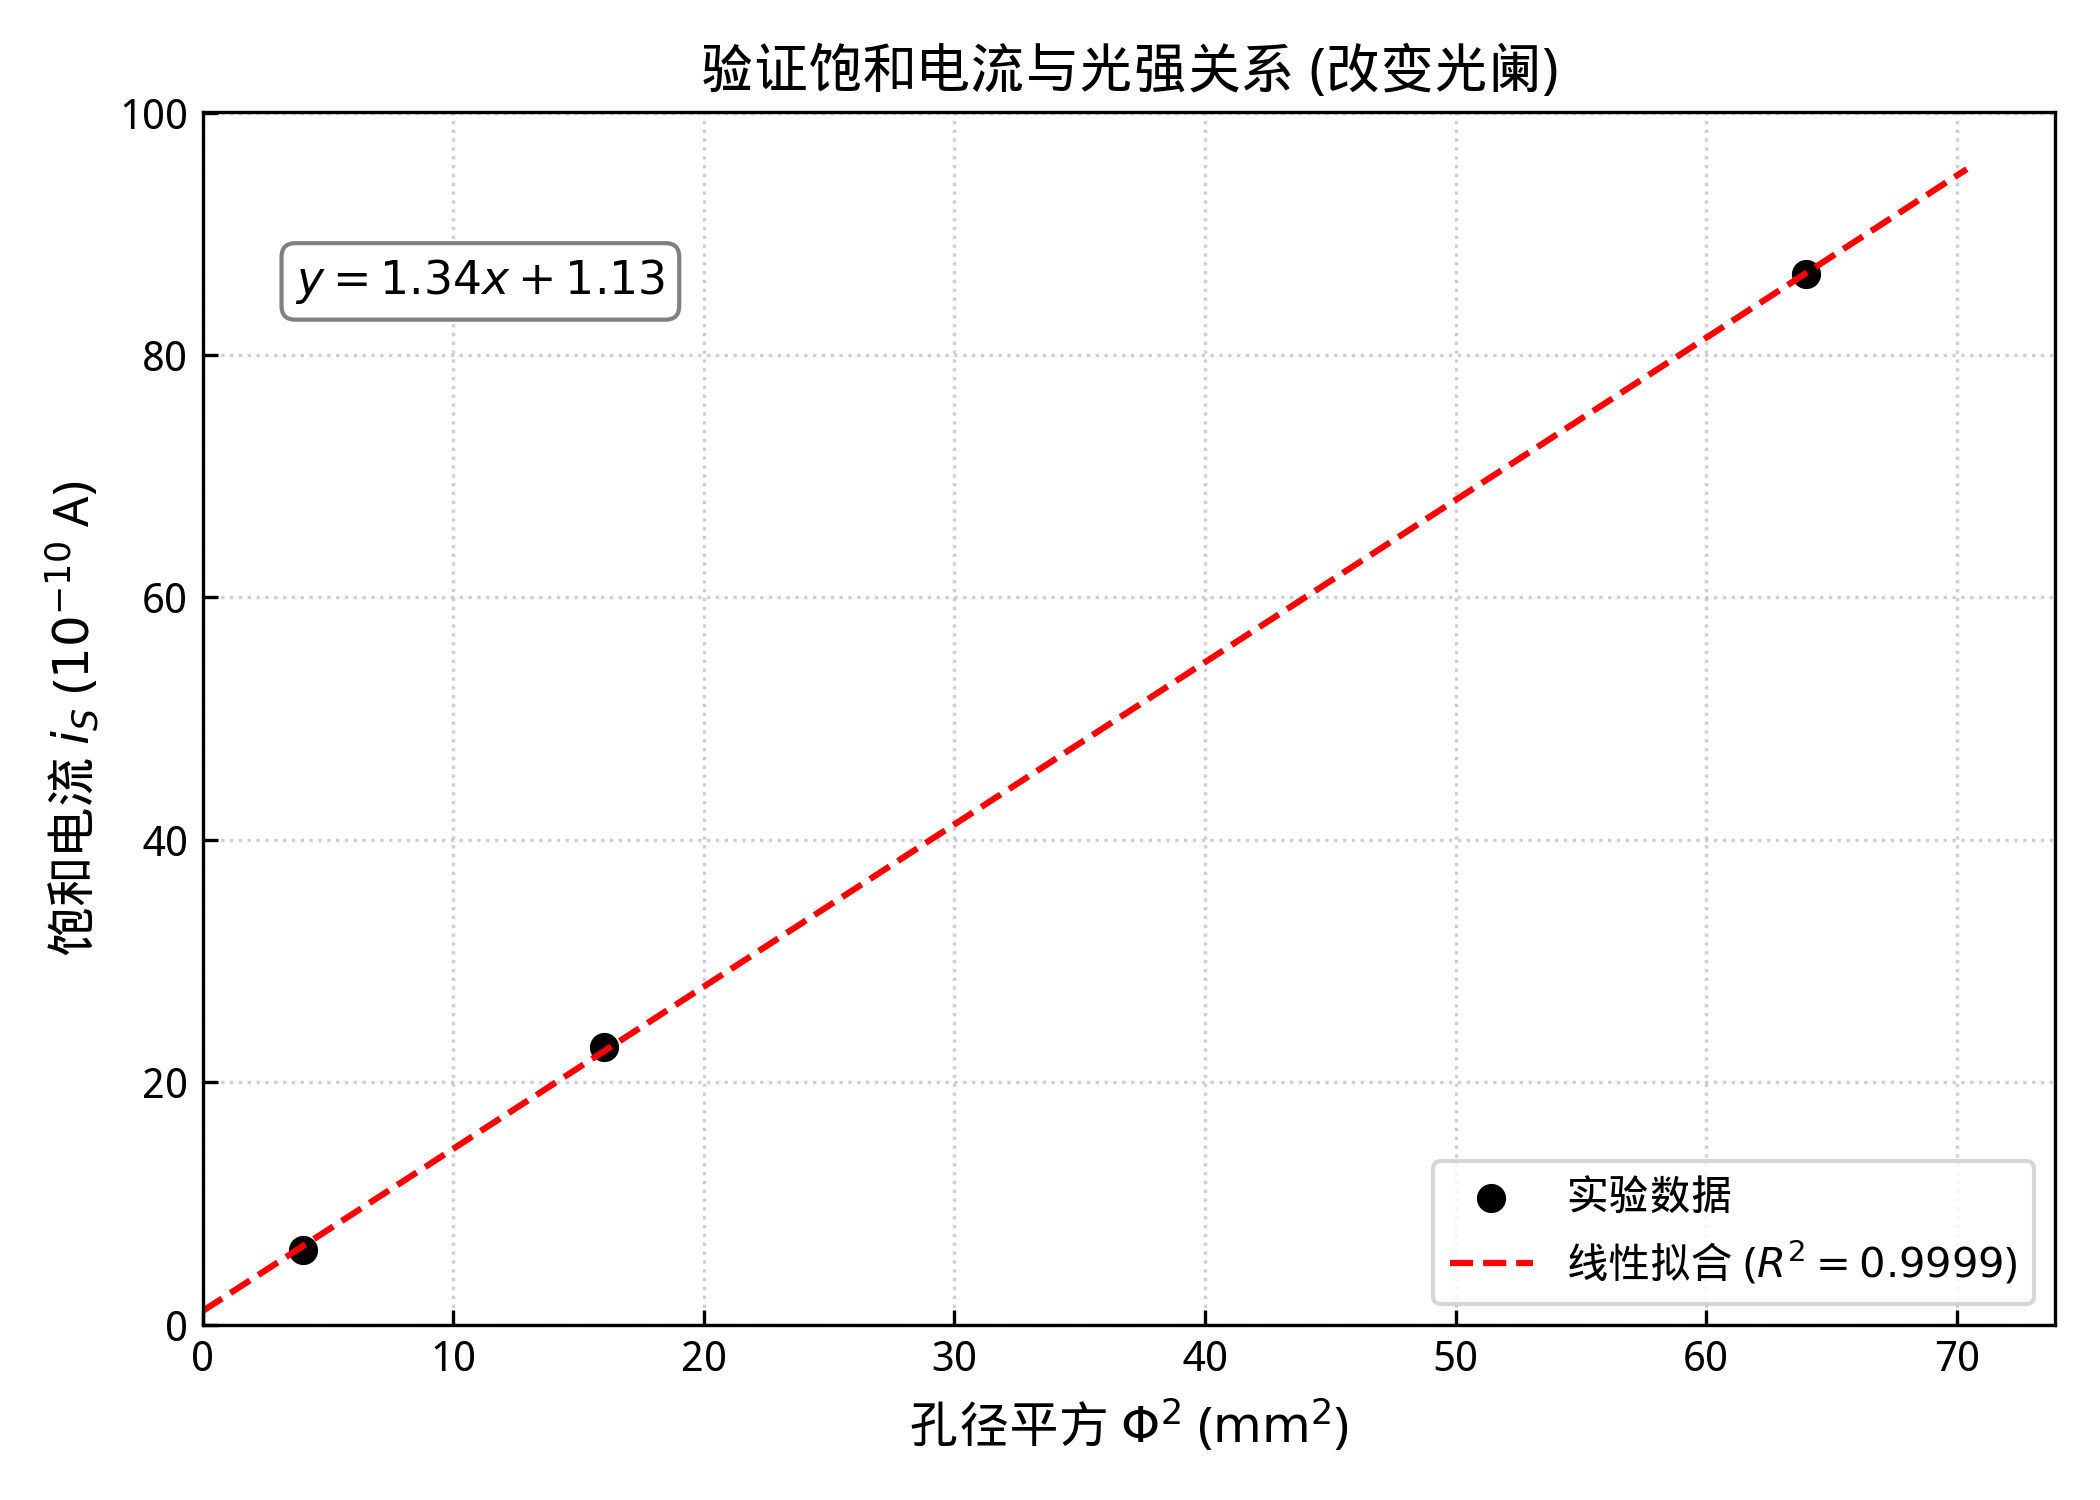
\includegraphics[width=0.8\linewidth]{./figures/saturation_aperture.png}
    \caption{饱和电流 $i_S$ 与光阑孔径平方 $\Phi^2$ 的关系}
    \label{fig:sat_aper}
\end{figure}

如图 \ref{fig:sat_aper} 所示，三个实验点与拟合直线的线性相关度极高（$R^2 \approx 0.999$）。这表明饱和电流与光阑孔径的平方成正比，进一步验证了光电管的饱和电流与入射光强成正比的结论。


    \subsection{误差分析}
    \xiaosi （运用测量误差、相对误差、不确定度等分析实验结果，20分）
    
    \begin{enumerate}
        \item 本实验仪器存在\(1 \sim  2×10^{-14}A\)的暗电流，一定程度上影响了对遏止电压\(U_a\)的准确测量，造成一定误差；
        \item 在实验中光电管输出电流表的读数并不稳定，不时会发生变化，给测量带来一定误差；
        \item 本实验中，虽提前对相关仪器进行了预热，但温度漂移的影响难以完全消除，会给读数造成影响，产生一定误差；
        \item 汞灯产生的光强受许多因素影响，不会一直保持恒定值，而是会有浮动，造成一定误差；
        \item 实际透过滤光片的光波长与 5 个对应的标称值可能不完全相同，存在一定偏差，给 $h$ 的计算带来误差。
    \end{enumerate}   
    
    \subsection{实验探讨}
    \xiaosi （对实验内容、现象和过程的小结，不超过100字，10分）

    \myspace{1}

    本次实验我们使用精密仪器，努力地完成了实验操作，并在数据记录时认真仔细，通过对实验数据的处理和分析，深入理解了光电效应的原理及普朗克常数的测定方法。实验过程中，我们体会到了严谨的实验态度和规范的操作步骤对实验结果的重要性，同时也认识到了实验误差存在的客观性以及减小误差的多种方法。
    \section{思考题}

    \xiaosi （解答教材或讲义或老师布置的思考题，10分）

    \subsubsection*{测定普朗克常数的关键是什么？怎样根据光电管的特性曲线选择测定遏止电压\(U_a\)的方法？}

    \textbf{答：}测定普朗克常数的关键是获得单一频率的光（单色光），以及对遏止电压\(U_a\)的正确测量。通过对多种不同频率单色光的截止电压的测量，绘制\(U_a - \nu\)图，计算其斜率，根据\(h = ke\)，计算 $h$。
  
    准备一个可调的负压电源并连接光电管，随着负电压源电压绝对值的增大，光电流逐渐减小，记录光电流恰好减小至 0 时的 $U_{AK}$ 即为遏止电压\(U_a\)；实际测量中，光电管并非理想光电管，其阳极被少量阴极表面的低逸出功材料污染，被阴极反射过来的散射光照射后，产生阳极光电流，干扰\(U_a\)的测量；对于光电流特性为正向电流上升较快、反向电流很小的光电管，可以用光电流特性曲线与暗电流特性曲线交点的电位差\(U_a'\)近似当作遏止电位差\(U_a\)（交点法）；若反向特性曲线的反向电流虽然较大，但其饱和速度很快，则可用反向电流开始饱和时的拐点电位差\(U_a''\)当作遏止电位差\(U_a\)（拐点法）。
    
    \subsubsection*{从遏止电压\(U_a\)与入射光的频率\(\nu\)的关系曲线中你能确定阴极材料的逸出功\(W_0\)吗？}

    \textbf{答：}由公式\(U_a = \frac{h}{e}\nu - \frac{W_0}{e}\)可知，\(U_a - \nu\)图中直线截距\(b = -\frac{W_0}{e}\)，因此\(W_0 = -eb\)。

    \subsubsection*{本实验存在哪些误差来源？实验中如何解决这些问题？}

    \textbf{答：}误差来源详见误差分析。对于读数误差，可采用多次测量取平均值的方法减小误差，并采用精度更高的测量工具减少误差；可以采用精密仪器测量实际透过各滤光片的光波长，对测量结果进行修正；可采用交点法和拐点法测量\(U_a\)，减少阳极光电流对测量结果造成的误差。    

\newpage

\sihao\textbf{注意事项：}
\xiaosi
\begin{enumerate}
    \item  用 PDF 格式上传“实验报告”，文件名：学生姓名+学号+实验名称+周次。
    \item  “实验报告”必须递交在“学在浙大”的本课程的对应实验项目的“作业”模块内。
    \item  “实验报告”成绩必须在“浙江大学物理实验教学中心网站”-“选课系统”内查询。
    \item 教学评价必须在“浙江大学物理实验教学中心网站”-“选课系统”内进行，学生必须进行教学评价，才能看到实验报告成绩，教学评价必须在本次实验结束后 3 天内进行。
\end{enumerate}

\vspace{1cm}
\xiaosi\centering \textbf{浙江大学物理实验教学中心制}

\end{document}